
\section{Langkah-Langkah Percobaan}

Dalam percobaan routing \& manajemen IPv6, kami memulai dengan mempersiapkan peralatan yang dibutuhkan, yaitu dua buah PC sebagai \textit{end device} dan sebuah MikroTik sebagai router. Karena hanya menginginkan koneksi dan komunikasi antara dua \textit{end device}, maka tidak diperlukan \textit{switch}. Perangkat lunak yang digunakan untuk menghubungkan kedua router adalah Winbox. Seluruh konfigurasi router dilakukan melalui Winbox.


\subsection{Routing IPv6 Statis}
\begin{enumerate}
	\item  kedua \textit{end device} dihubungkan ke router yang tepat: \texttt{PC1 $\rightarrow$ Router\,1 — Router\,2 $\leftarrow$ PC2}.

\begin{figure}[H]
    \centering
    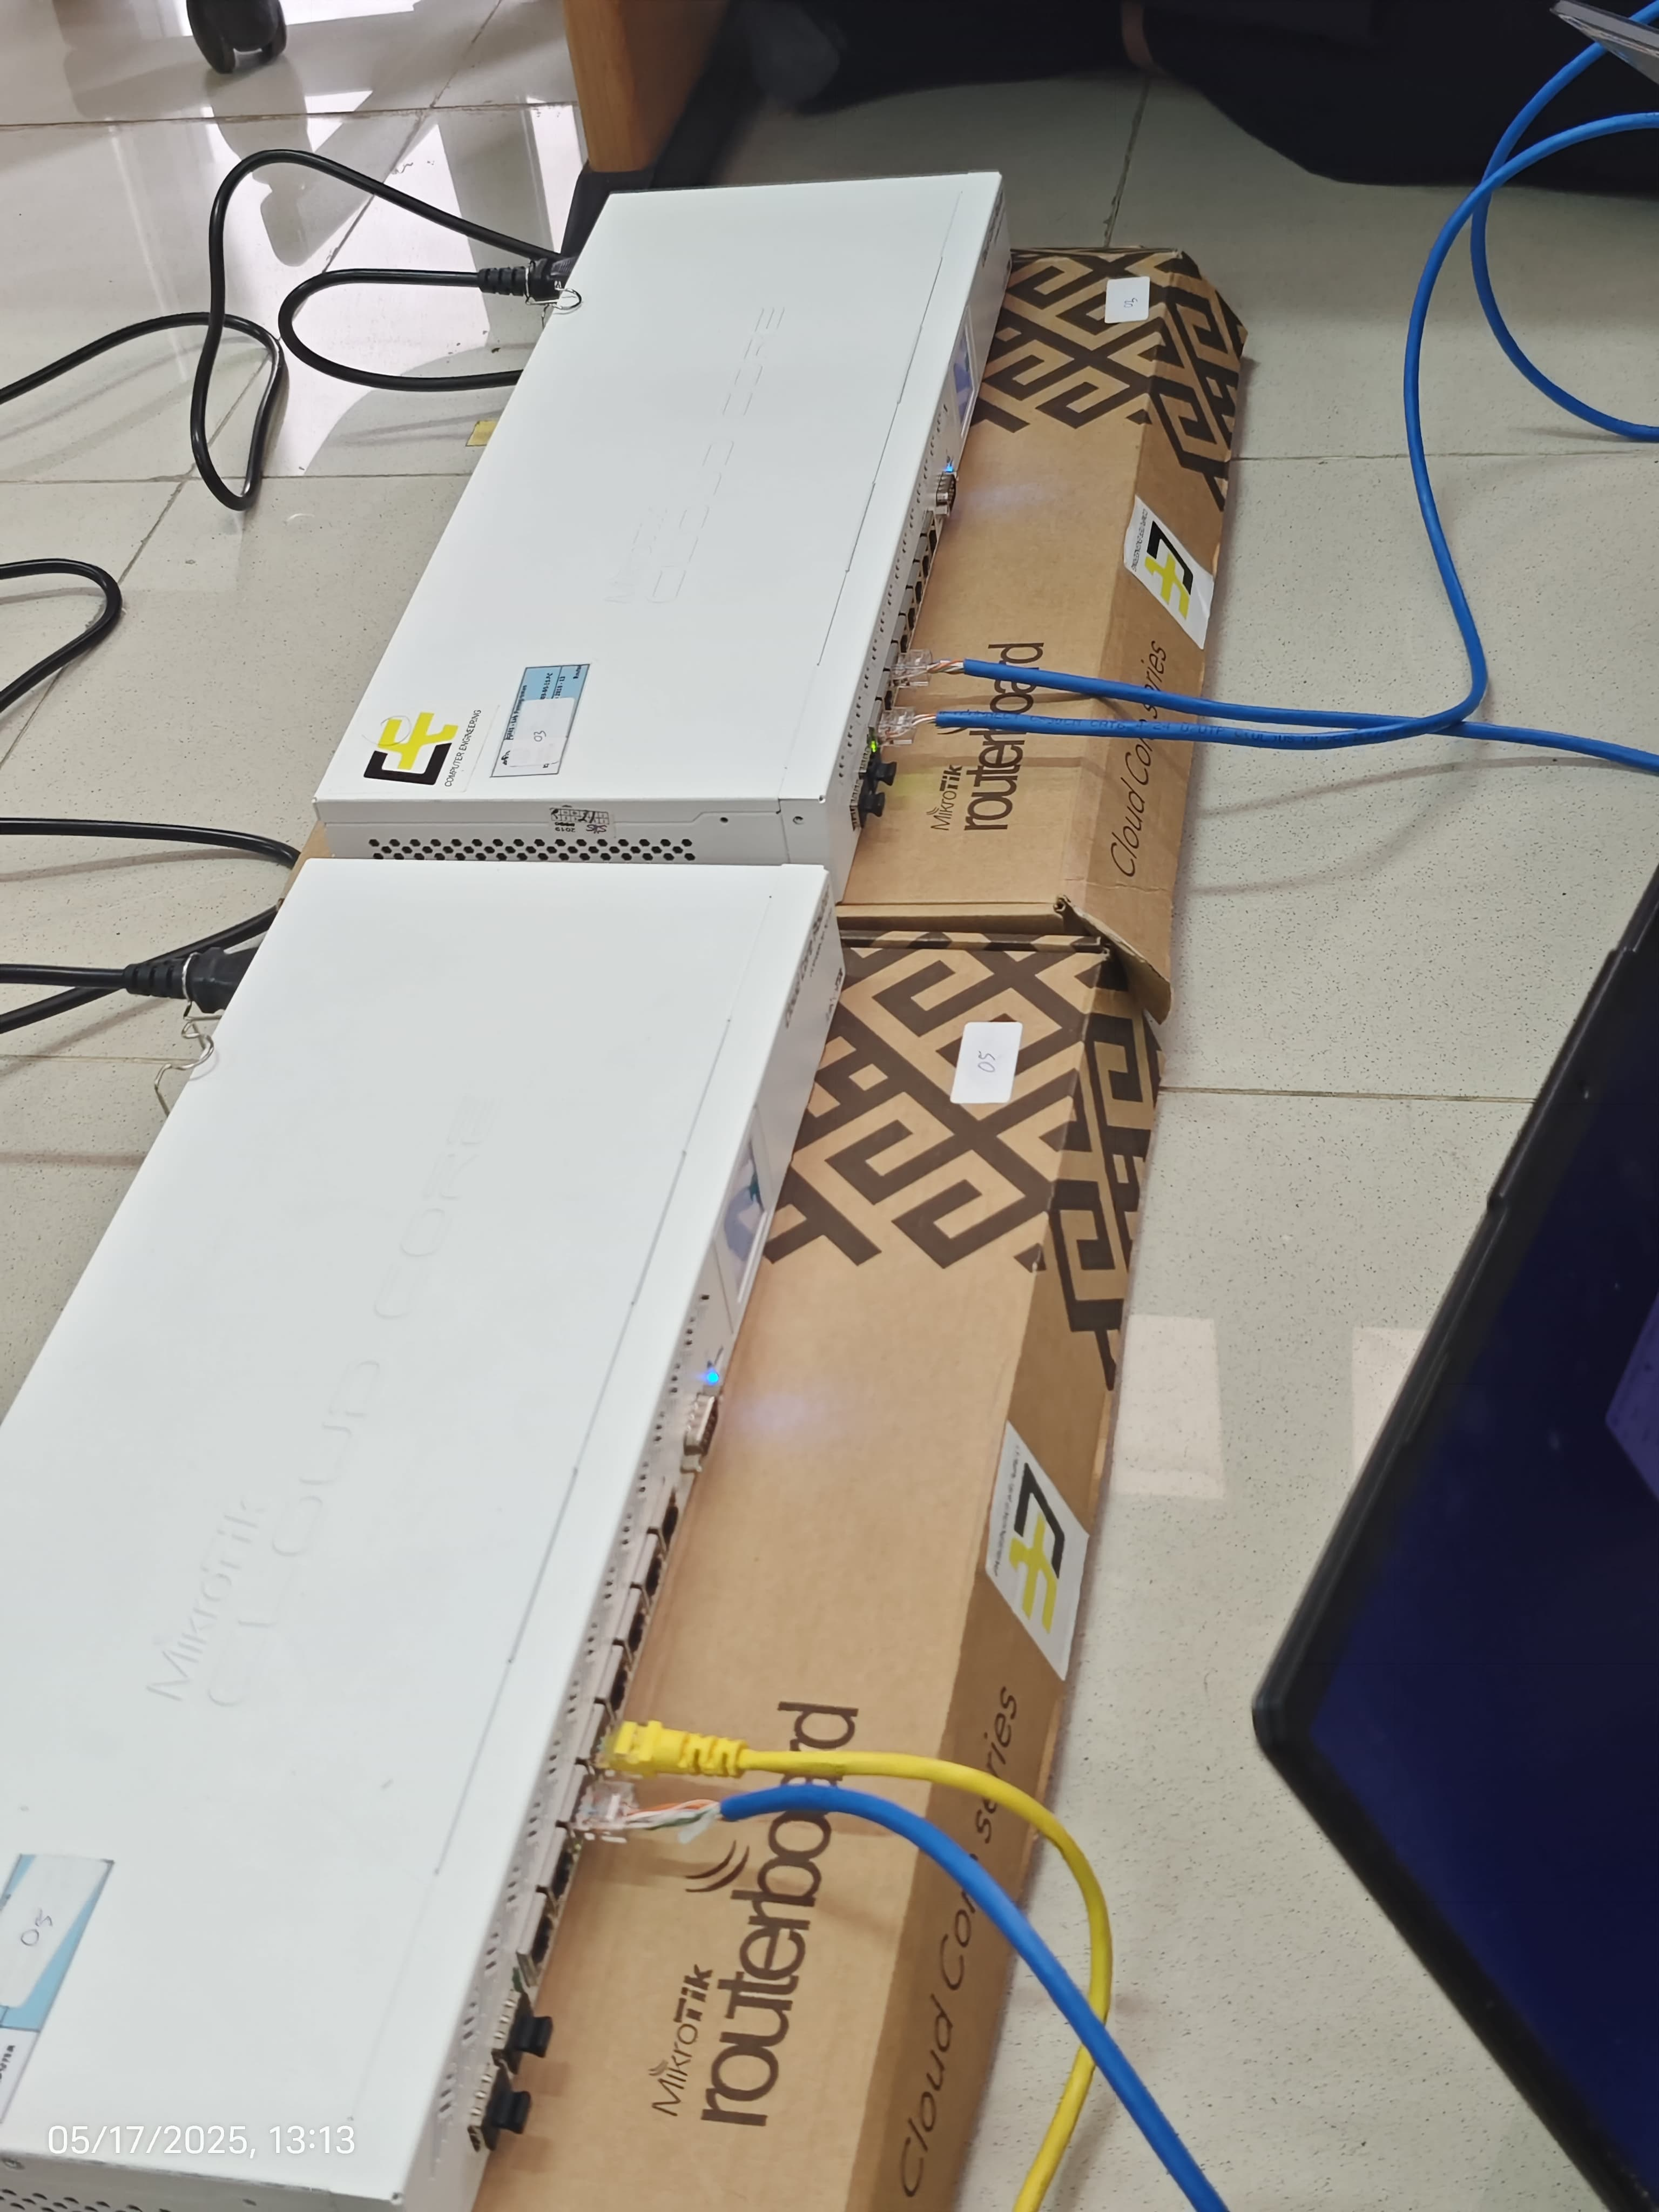
\includegraphics[width=0.48\textwidth]{img/Pasang.jpeg}
    \caption{Pemasangan kabel}
    \label{fig:pasang}
\end{figure}



\item Setelah terhubung secara fisik, buka Winbox untuk konfigurasi router.

\begin{figure}[H]
    \centering
    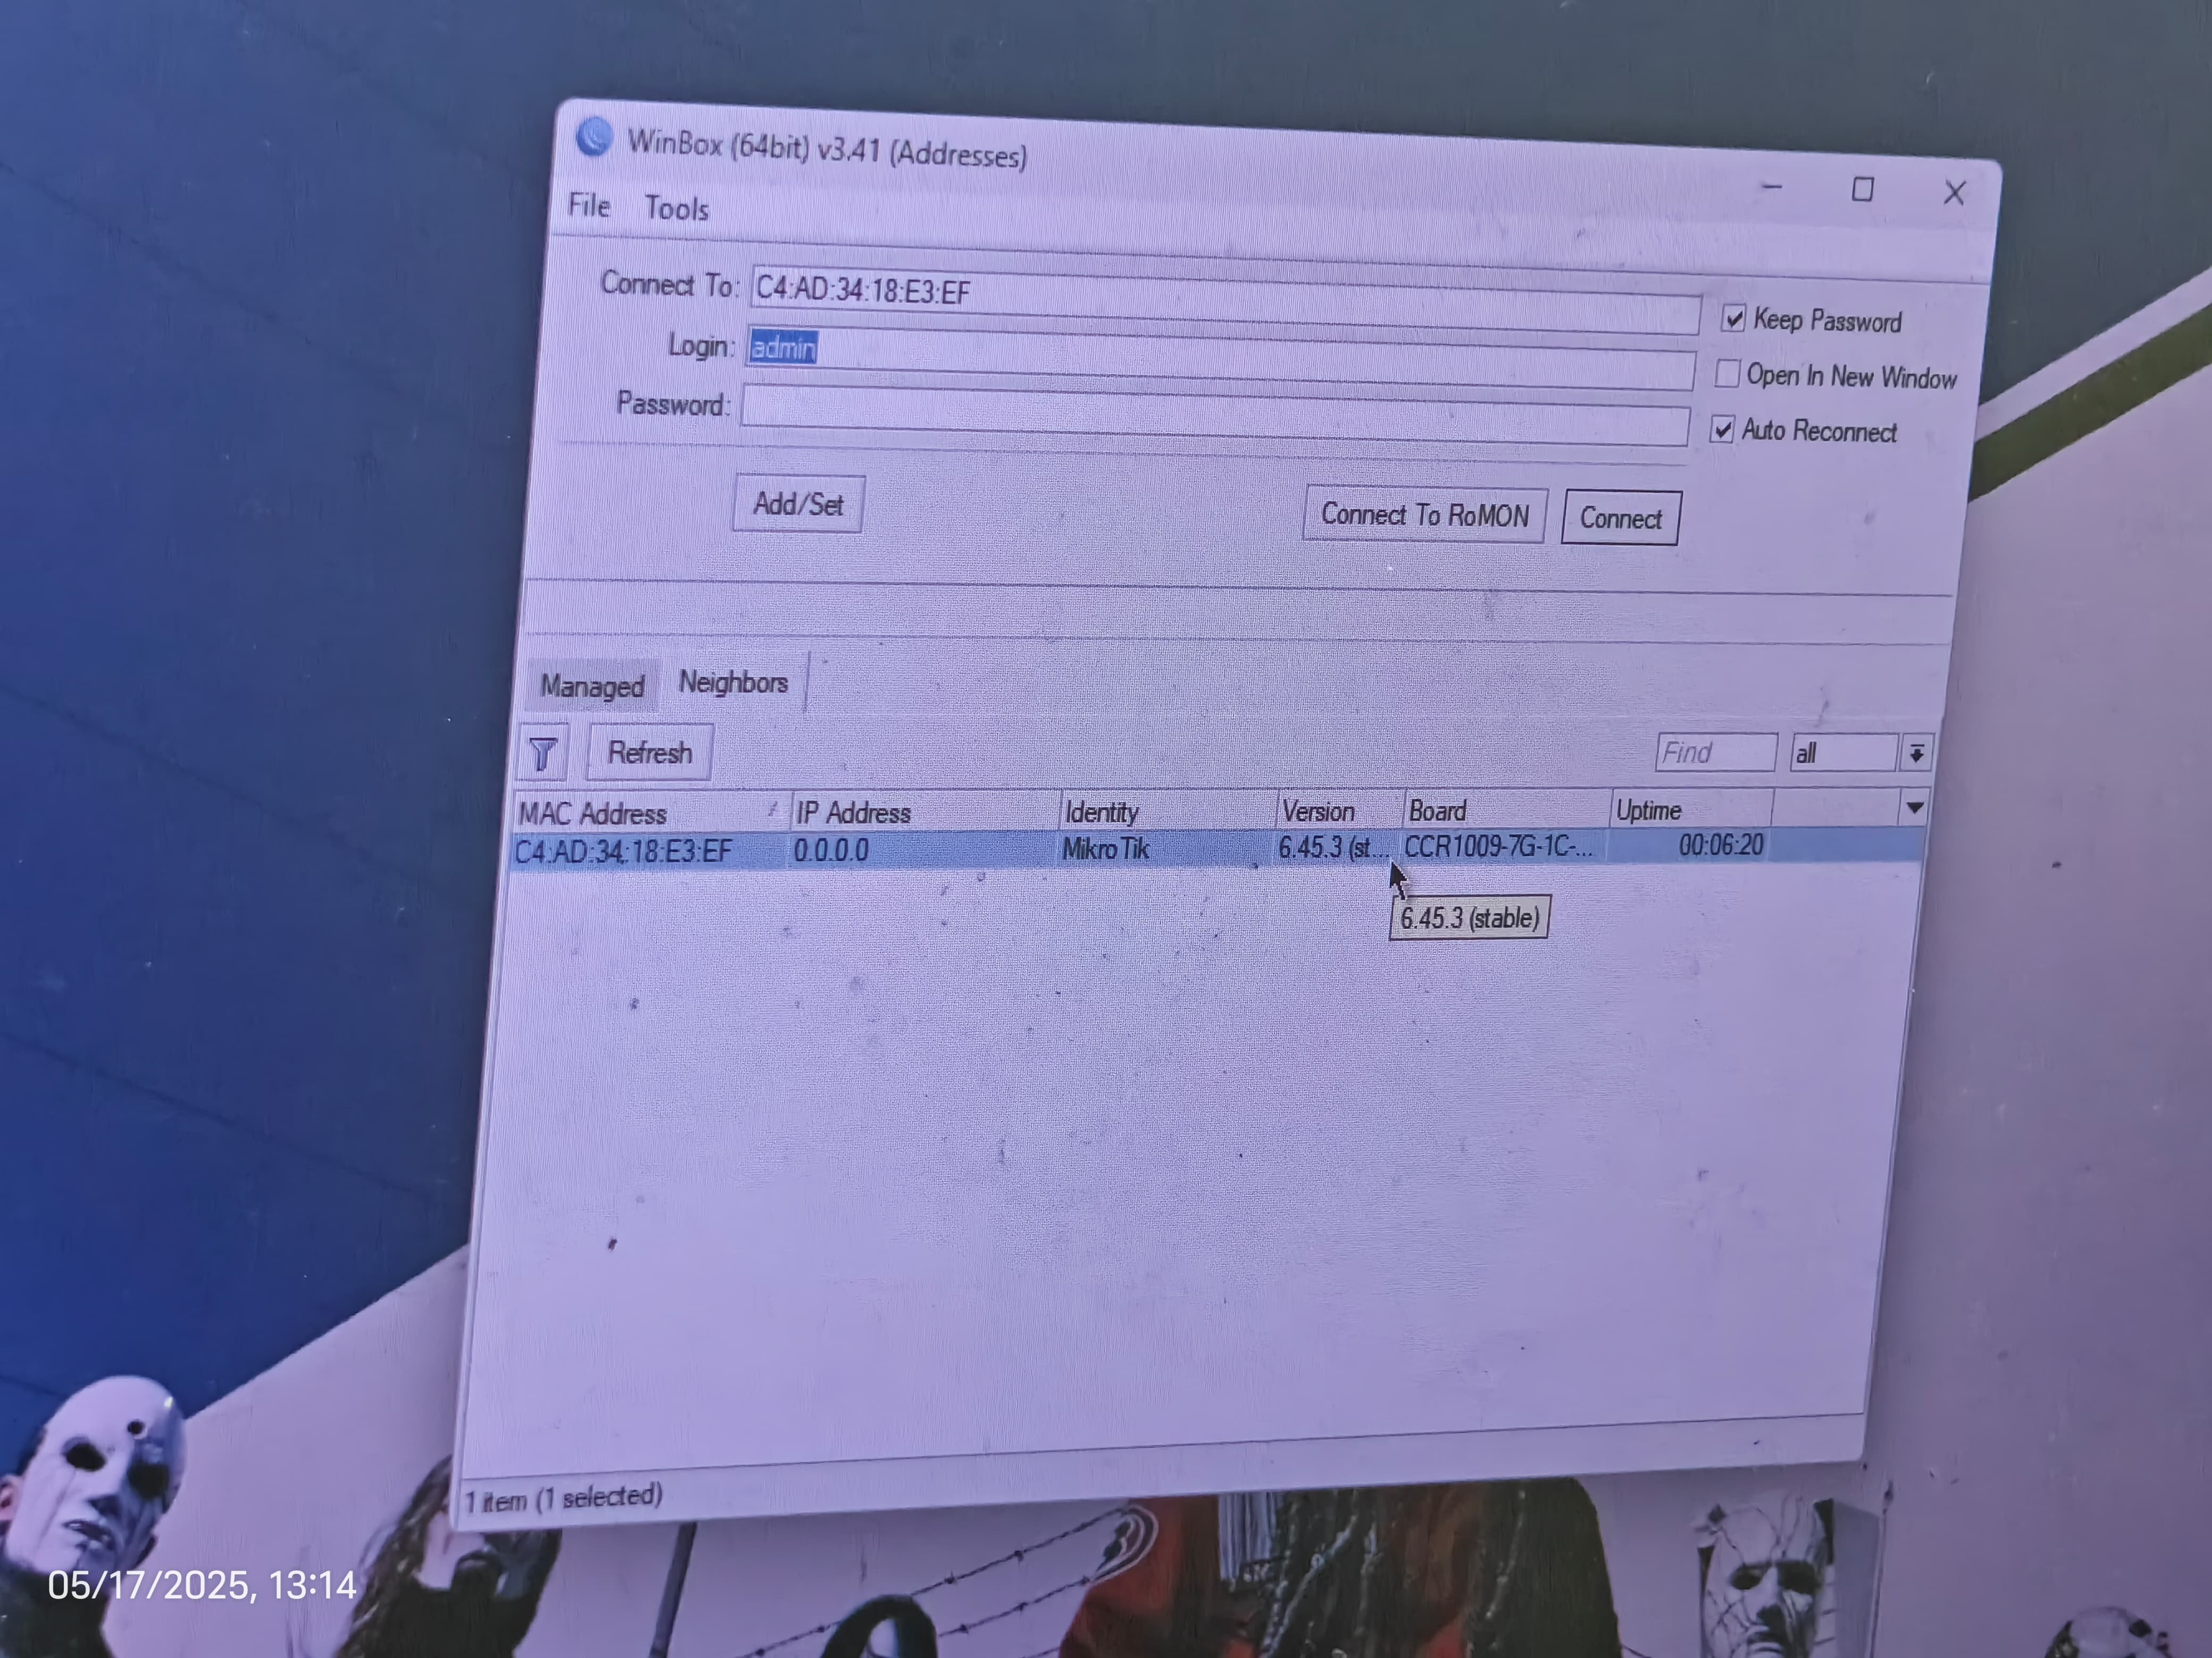
\includegraphics[width=0.48\textwidth]{img/winbox.jpeg}
    \caption{Masuk Winbox untuk konfigurasi router}
    \label{fig:winbox}
\end{figure}

\item Reset konfigurasi router untuk memastikan tidak ada bekas konfogurasi dari kelompok lainnya

\item Selanjutnya set IPv6 address PC.

\begin{figure}[H]
    \centering
    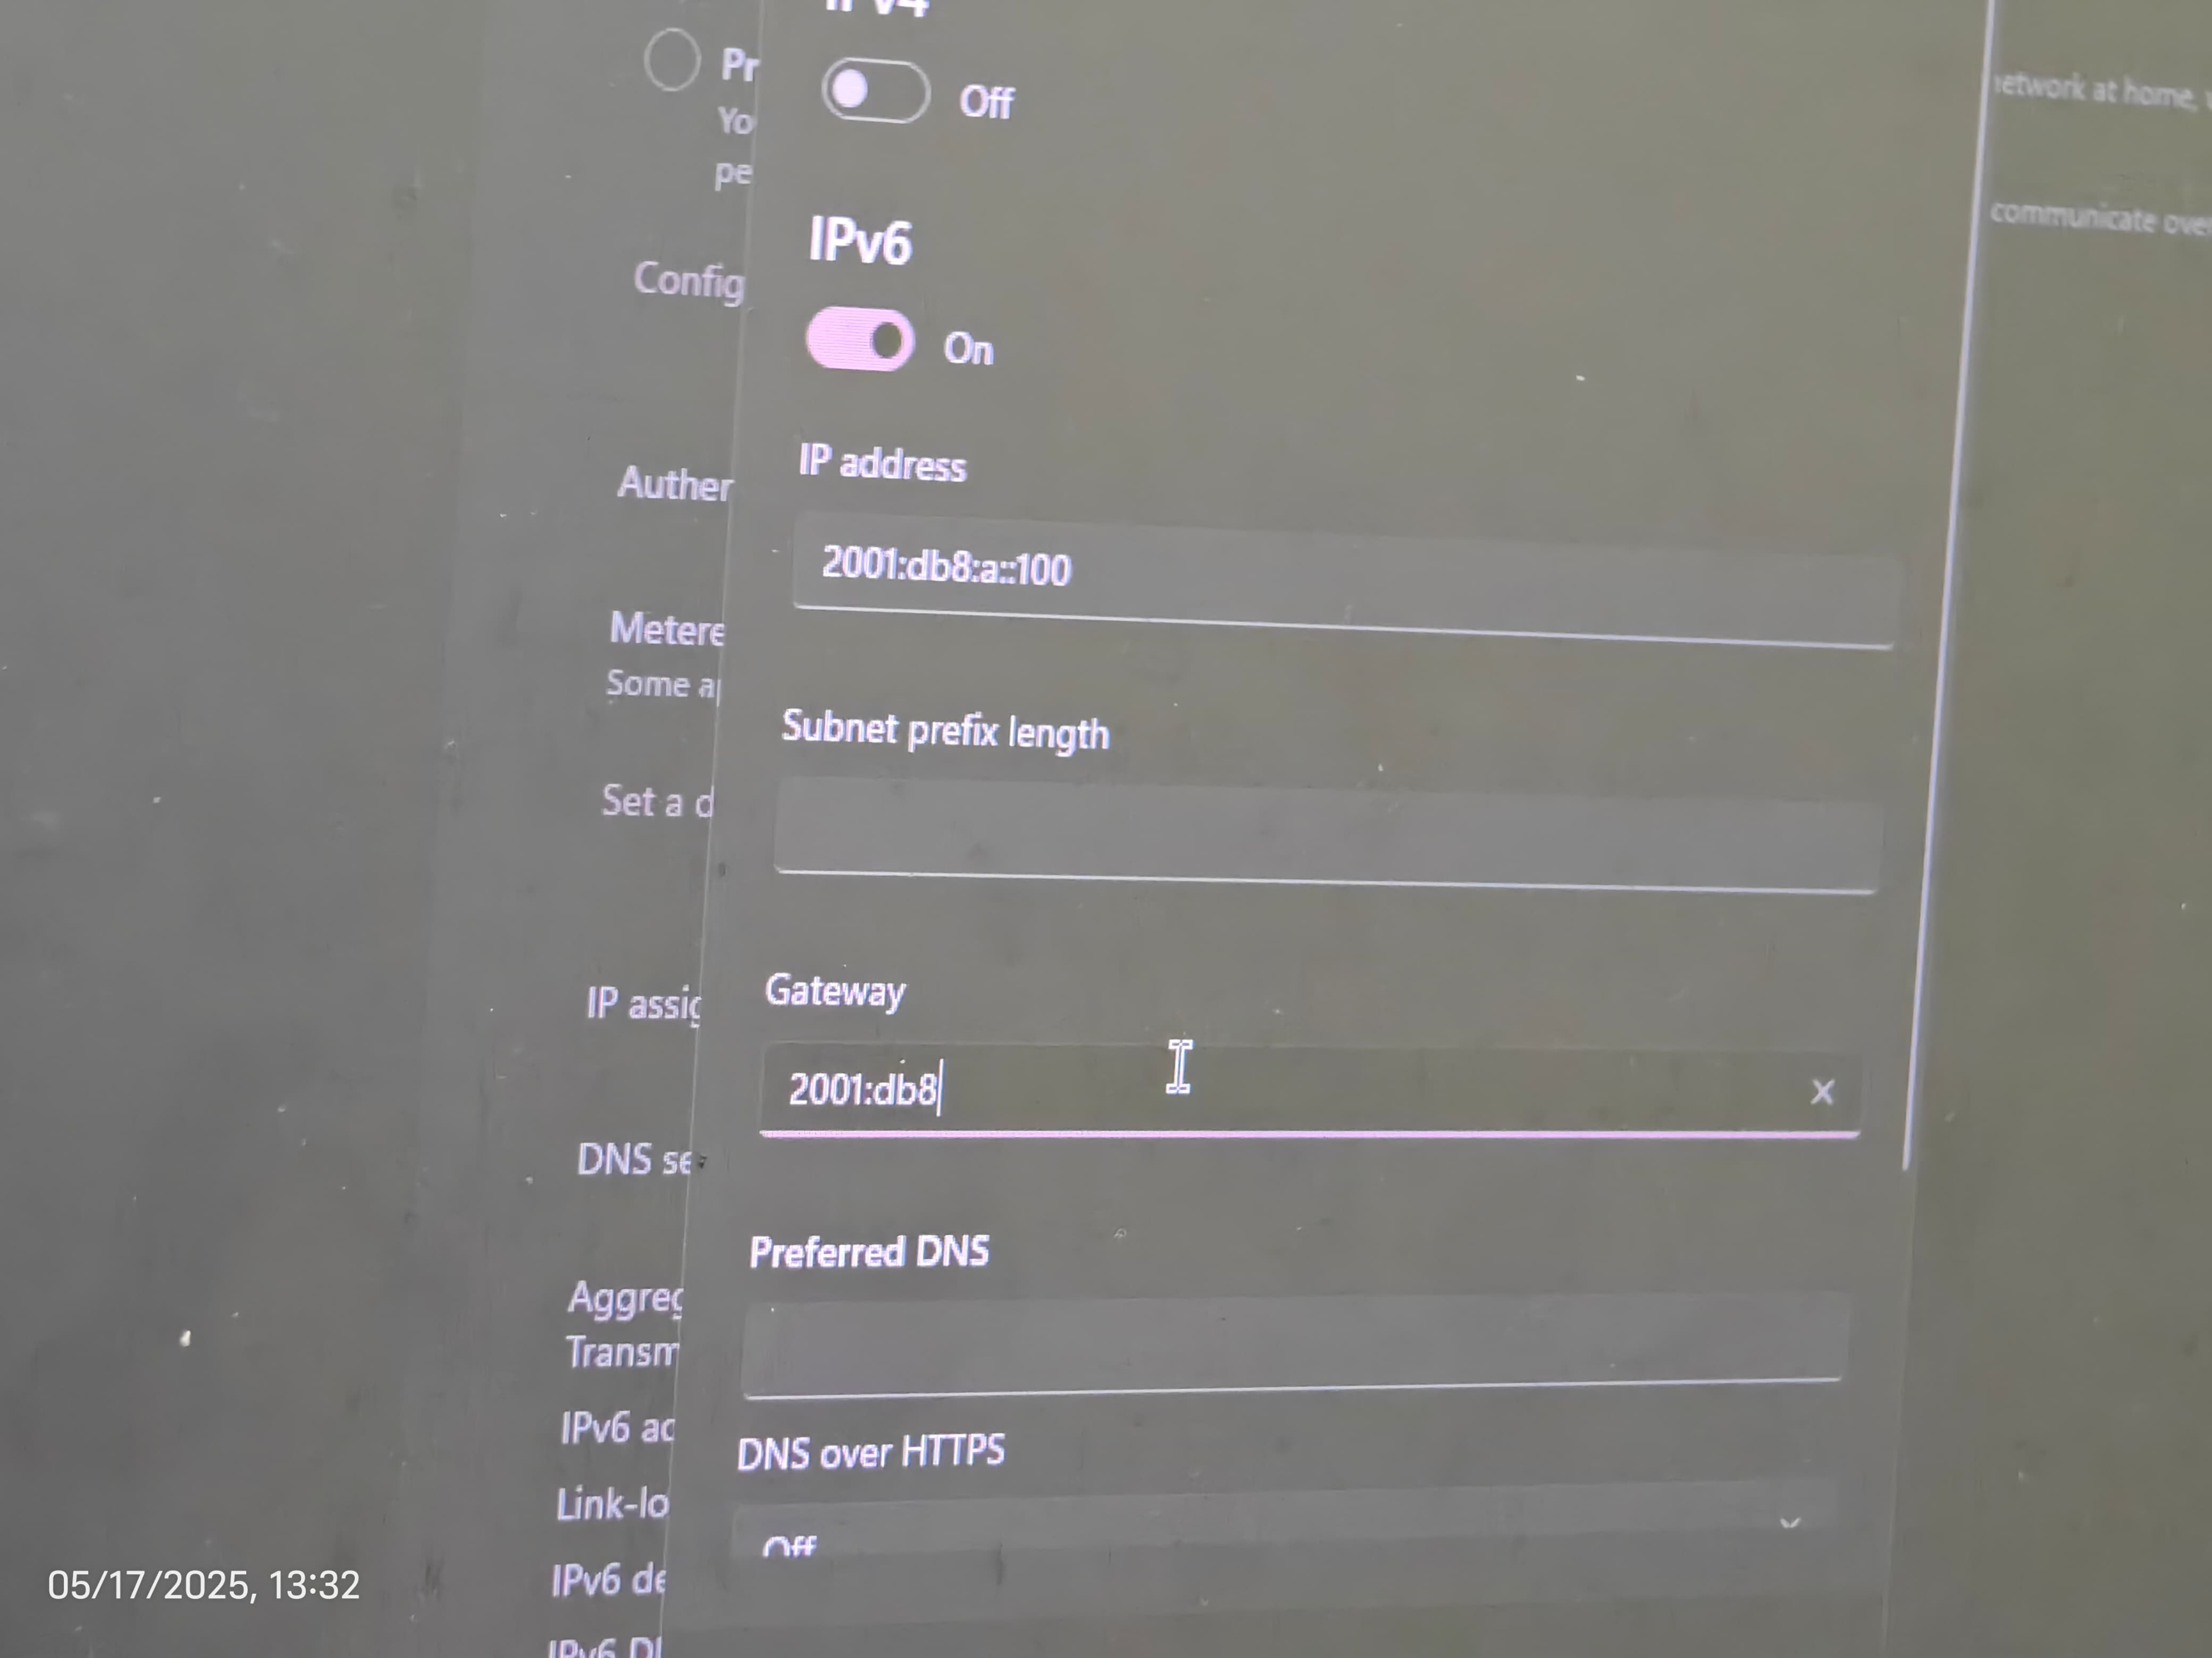
\includegraphics[width=0.48\textwidth]{img/address.jpeg}
    \caption{Address \textit{End Device}}
    \label{fig:address}
\end{figure}

\item Set IPv6 address untuk Router dan tambahkan address PC lainnya

\item Berikut konfigurasi \textit{address} untuk \textit{routing statis} IPv6. Tiga \textit{address} berikut ditujukan bagi Router\,1, Router\,2, dan PC2 (dengan asumsi \textit{end device} yang digunakan adalah PC1).

\begin{figure}[H]
    \centering
    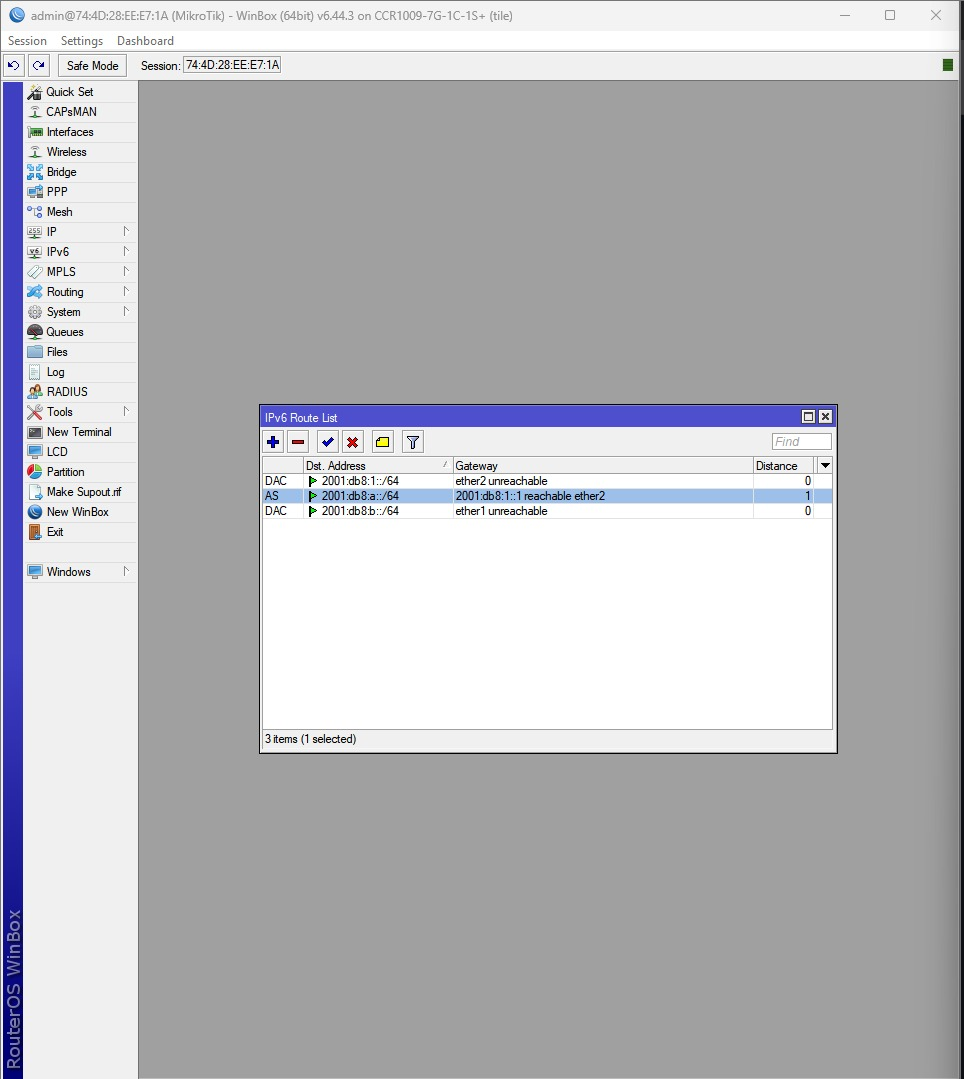
\includegraphics[width=0.48\textwidth]{img/A1.jpeg}
    \caption{Konfigurasi alamat}
    \label{fig:a1}
\end{figure}

\item lakukan uji \textit{ping} dari kedua \textit{end device}.

\begin{figure}[H]
    \centering
    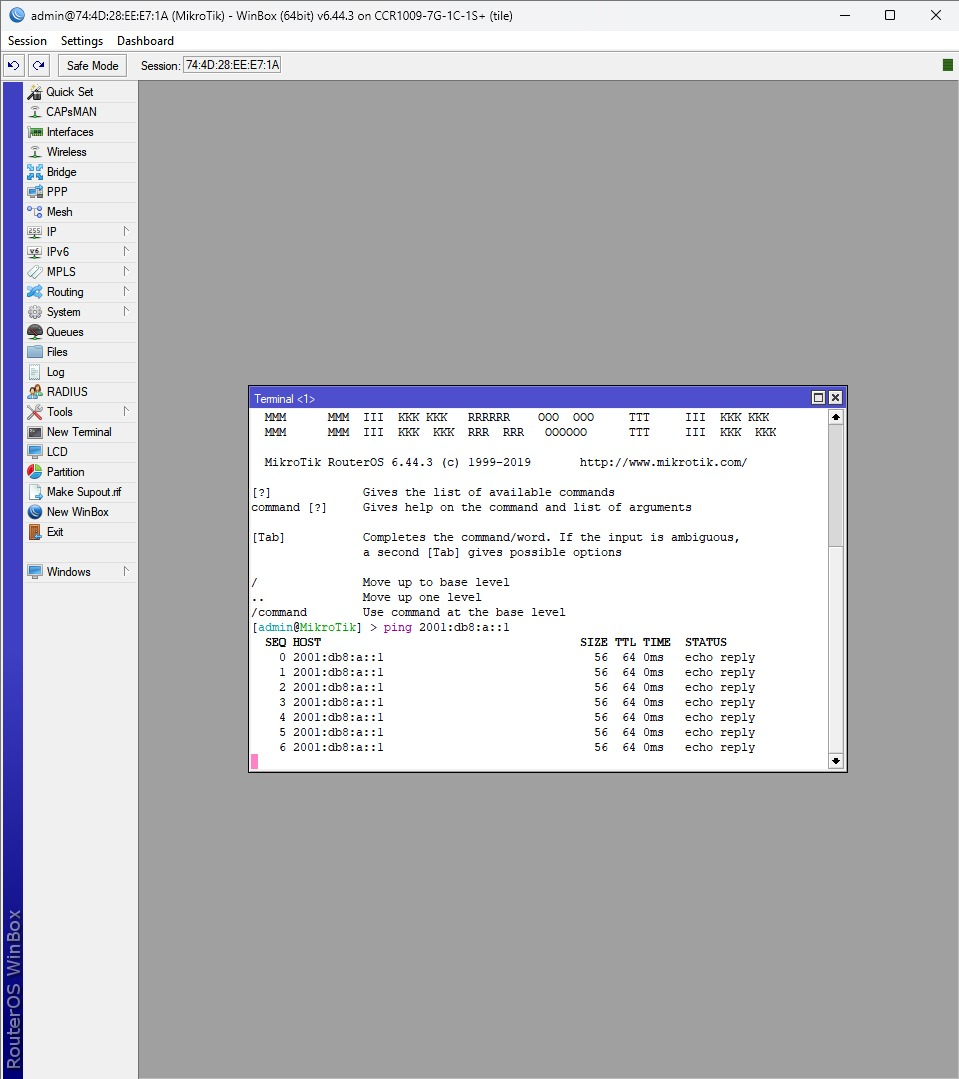
\includegraphics[width=0.48\textwidth]{img/A2.jpeg}
    \caption{Uji \textit{ping} dari PC1}
    \label{fig:a2a}
\end{figure}

\begin{figure}[H]
    \centering
    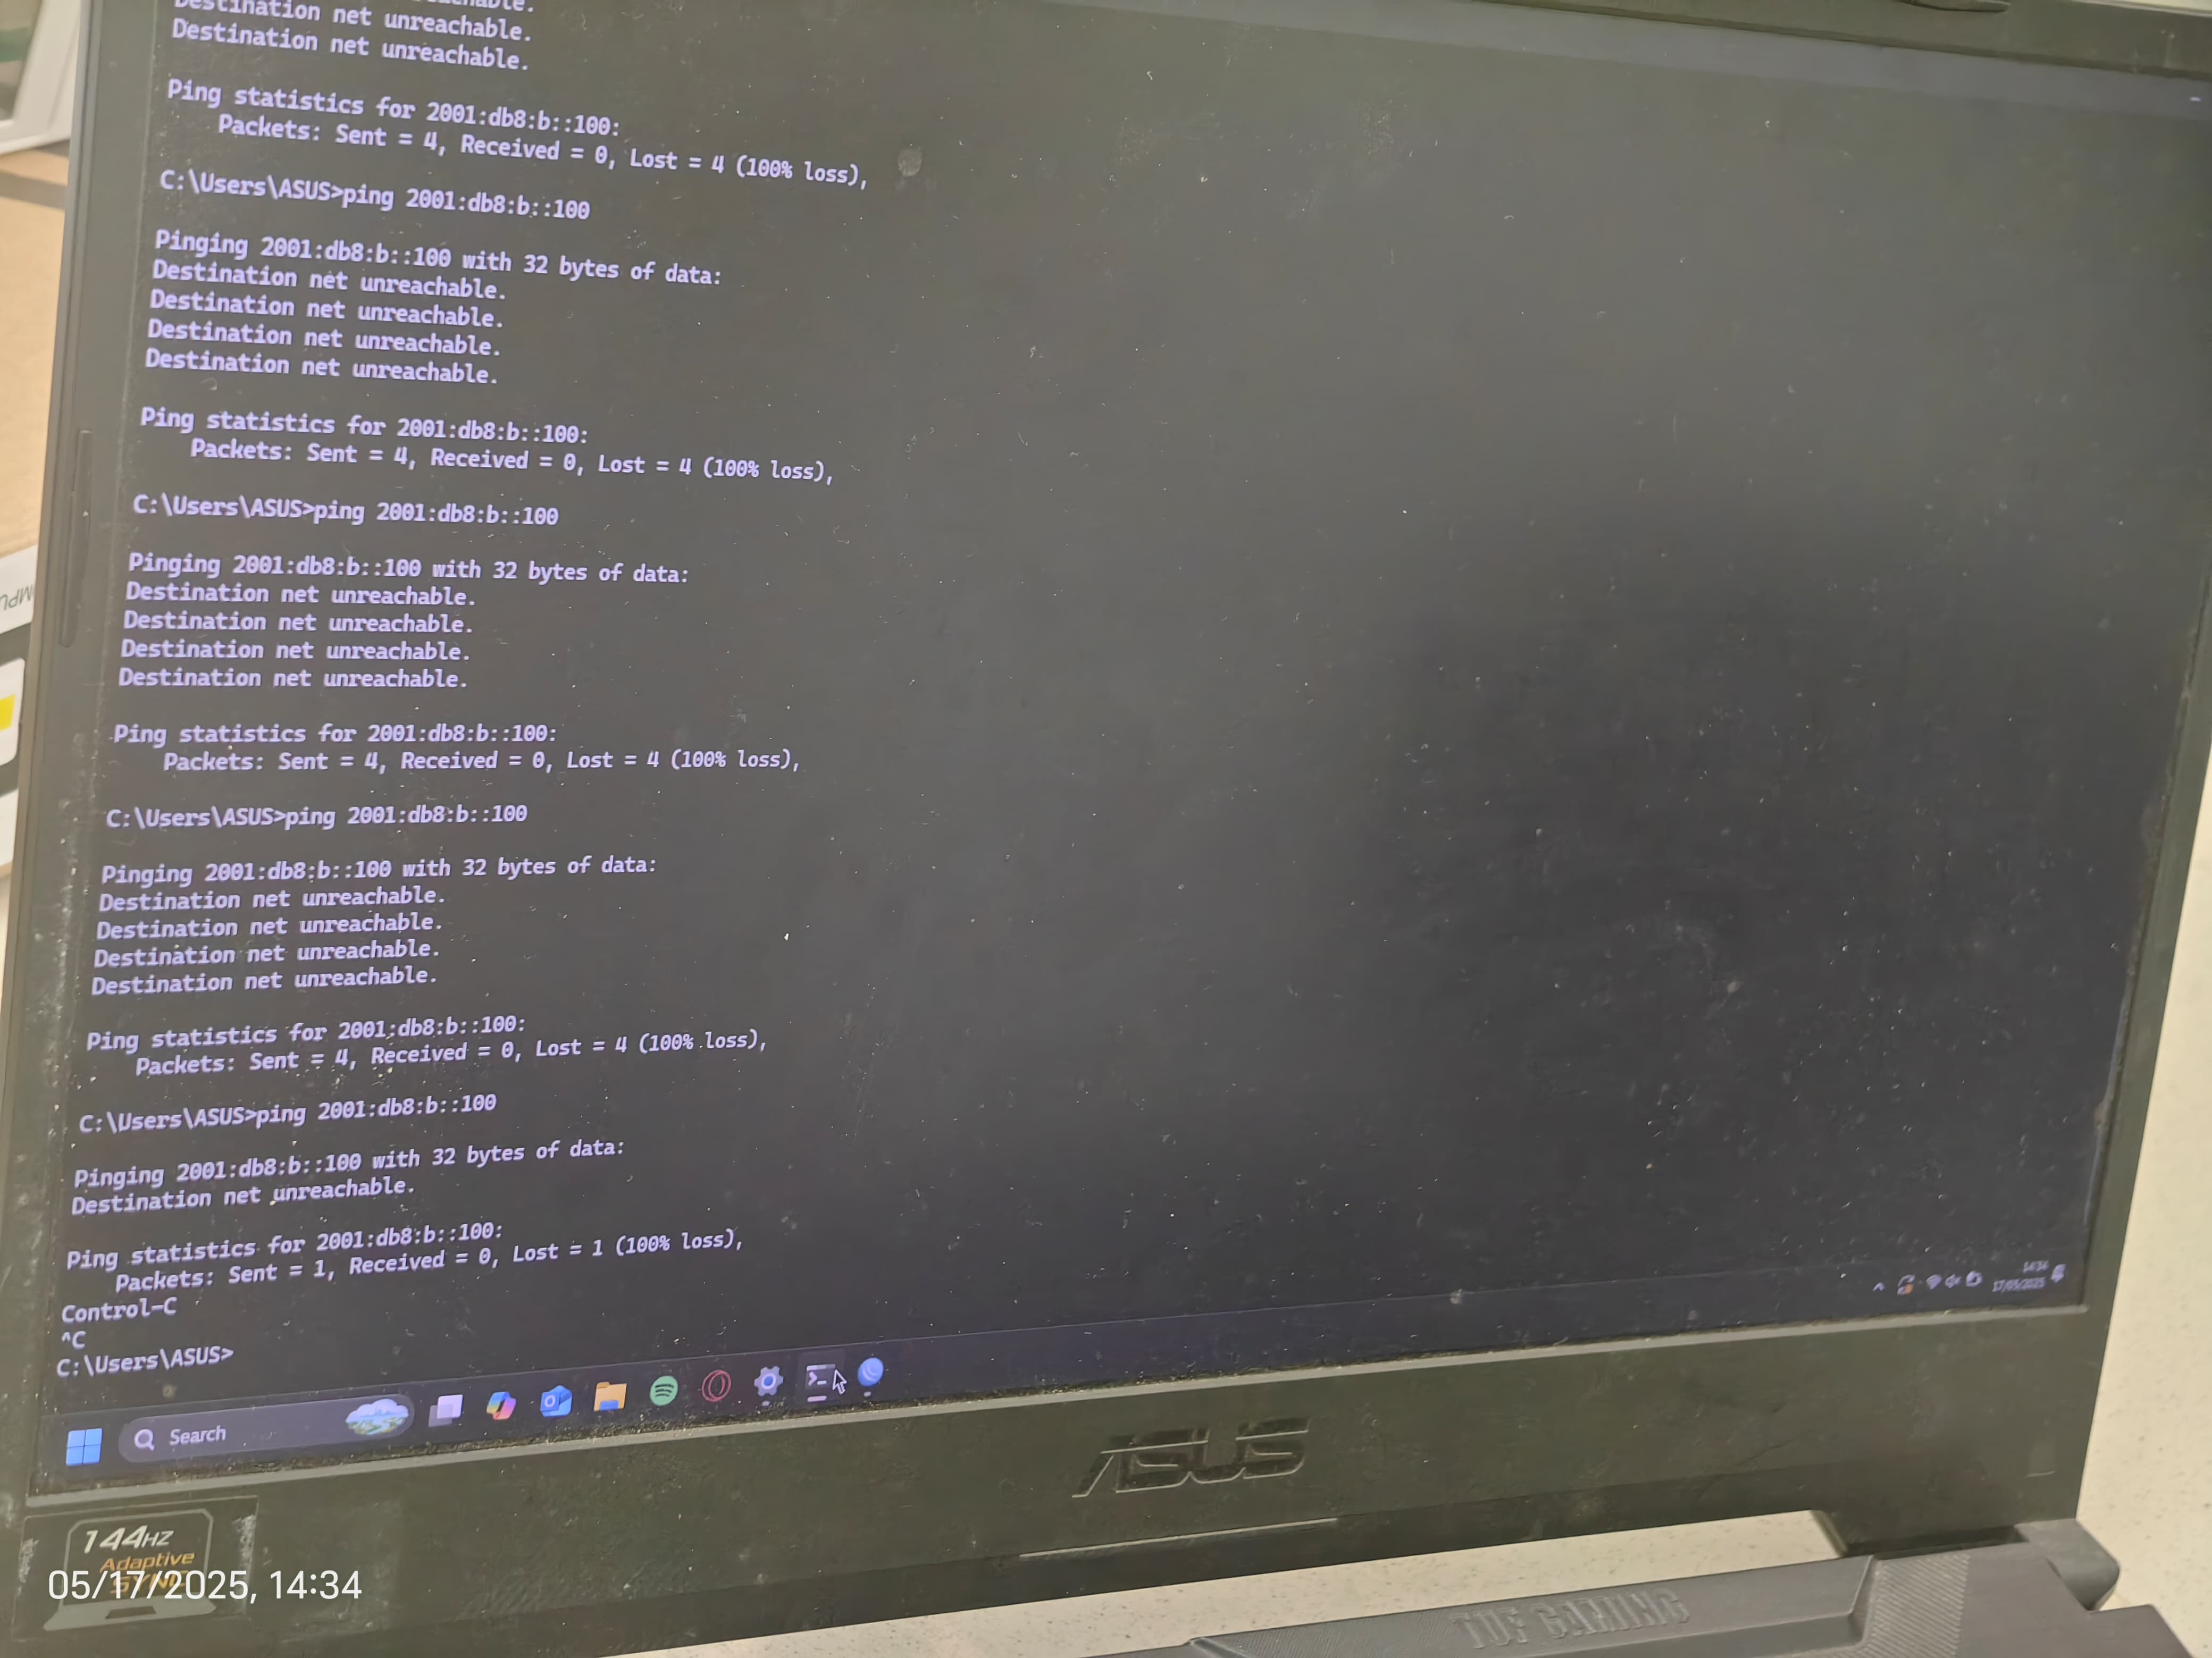
\includegraphics[width=0.48\textwidth]{img/A2-2.jpeg}
    \caption{Uji \textit{ping} dari PC2}
    \label{fig:a2b}
\end{figure}
\end{enumerate}

\newpage
\subsection{Routing IPv6 Dinamis}

\begin{enumerate}
\item Reset konfigurasi router
\item Set IP Address untuk Router dan PC.
\begin{figure}[H]
    \centering
    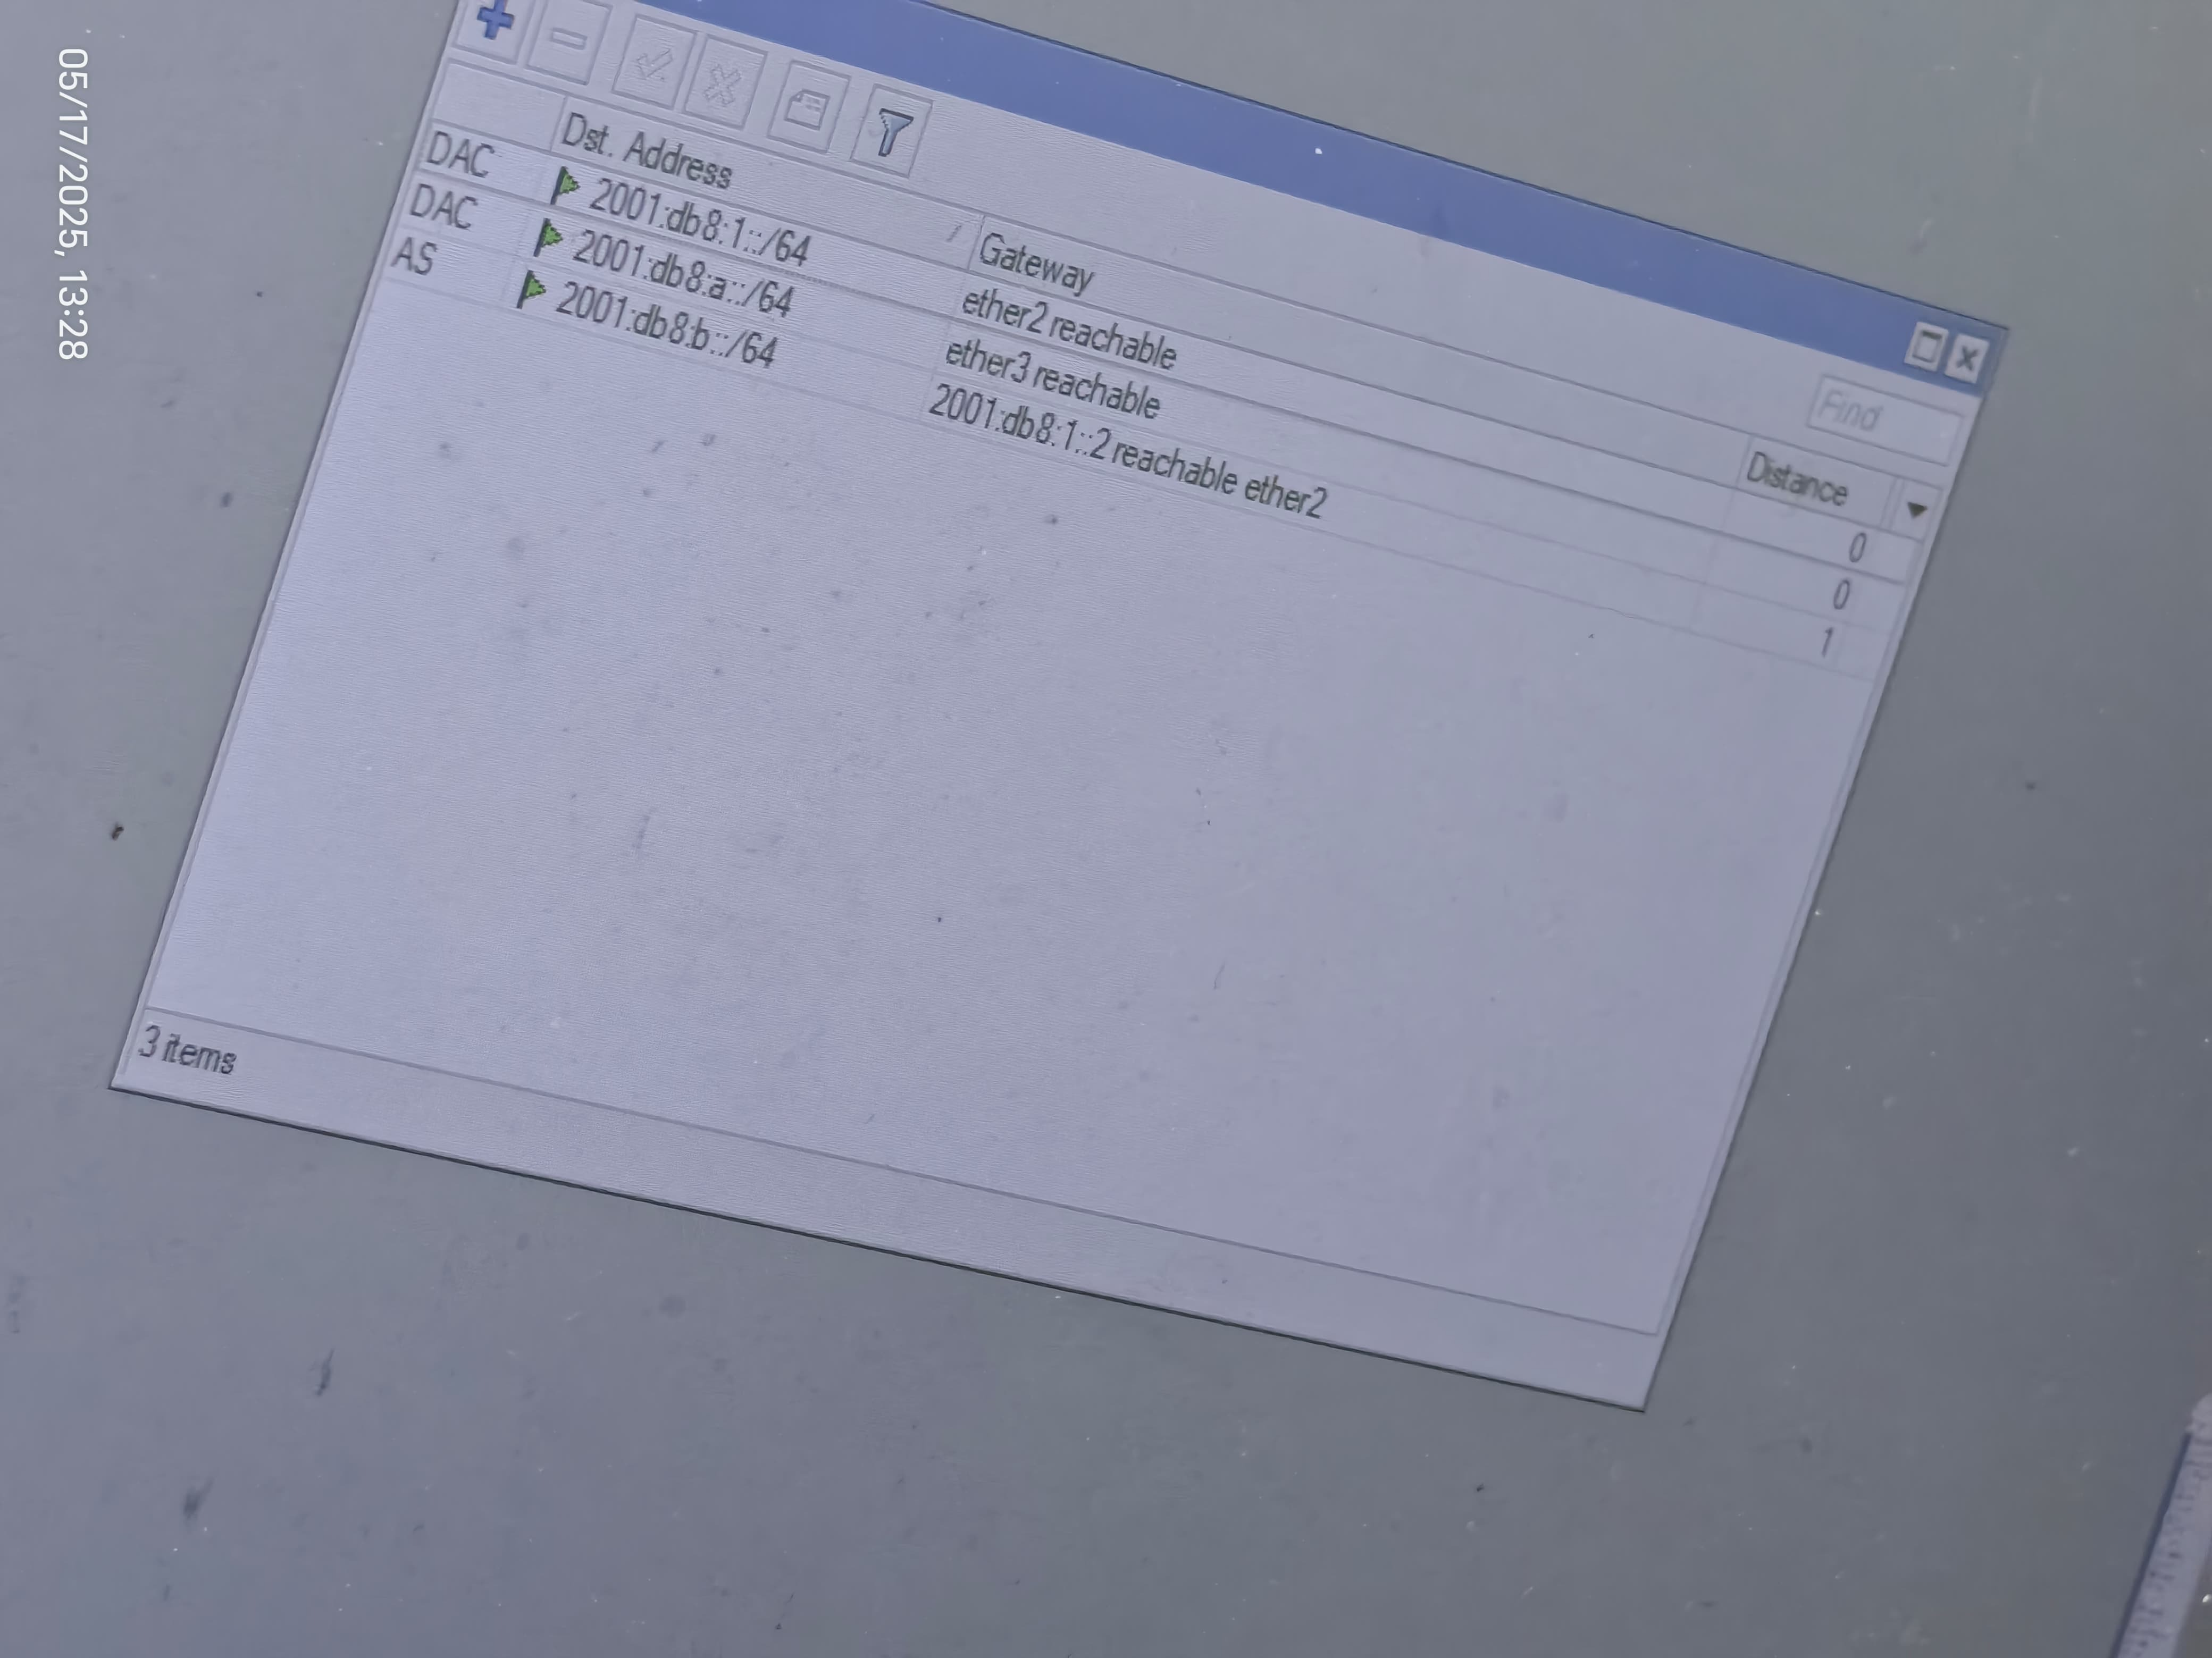
\includegraphics[width=0.48\textwidth]{img/A4.jpg}
    \caption{Konfigurasi alamat pada PC2}
    \label{fig:a4}
\end{figure}

\item Buat instance OSPFv3 untuk routing dinamis
\item cek Neighbor $\&$ Routing dan pastikan rute dinamis antar router tersedia

\item uji ping pada PC
\begin{figure}[H]
    \centering
    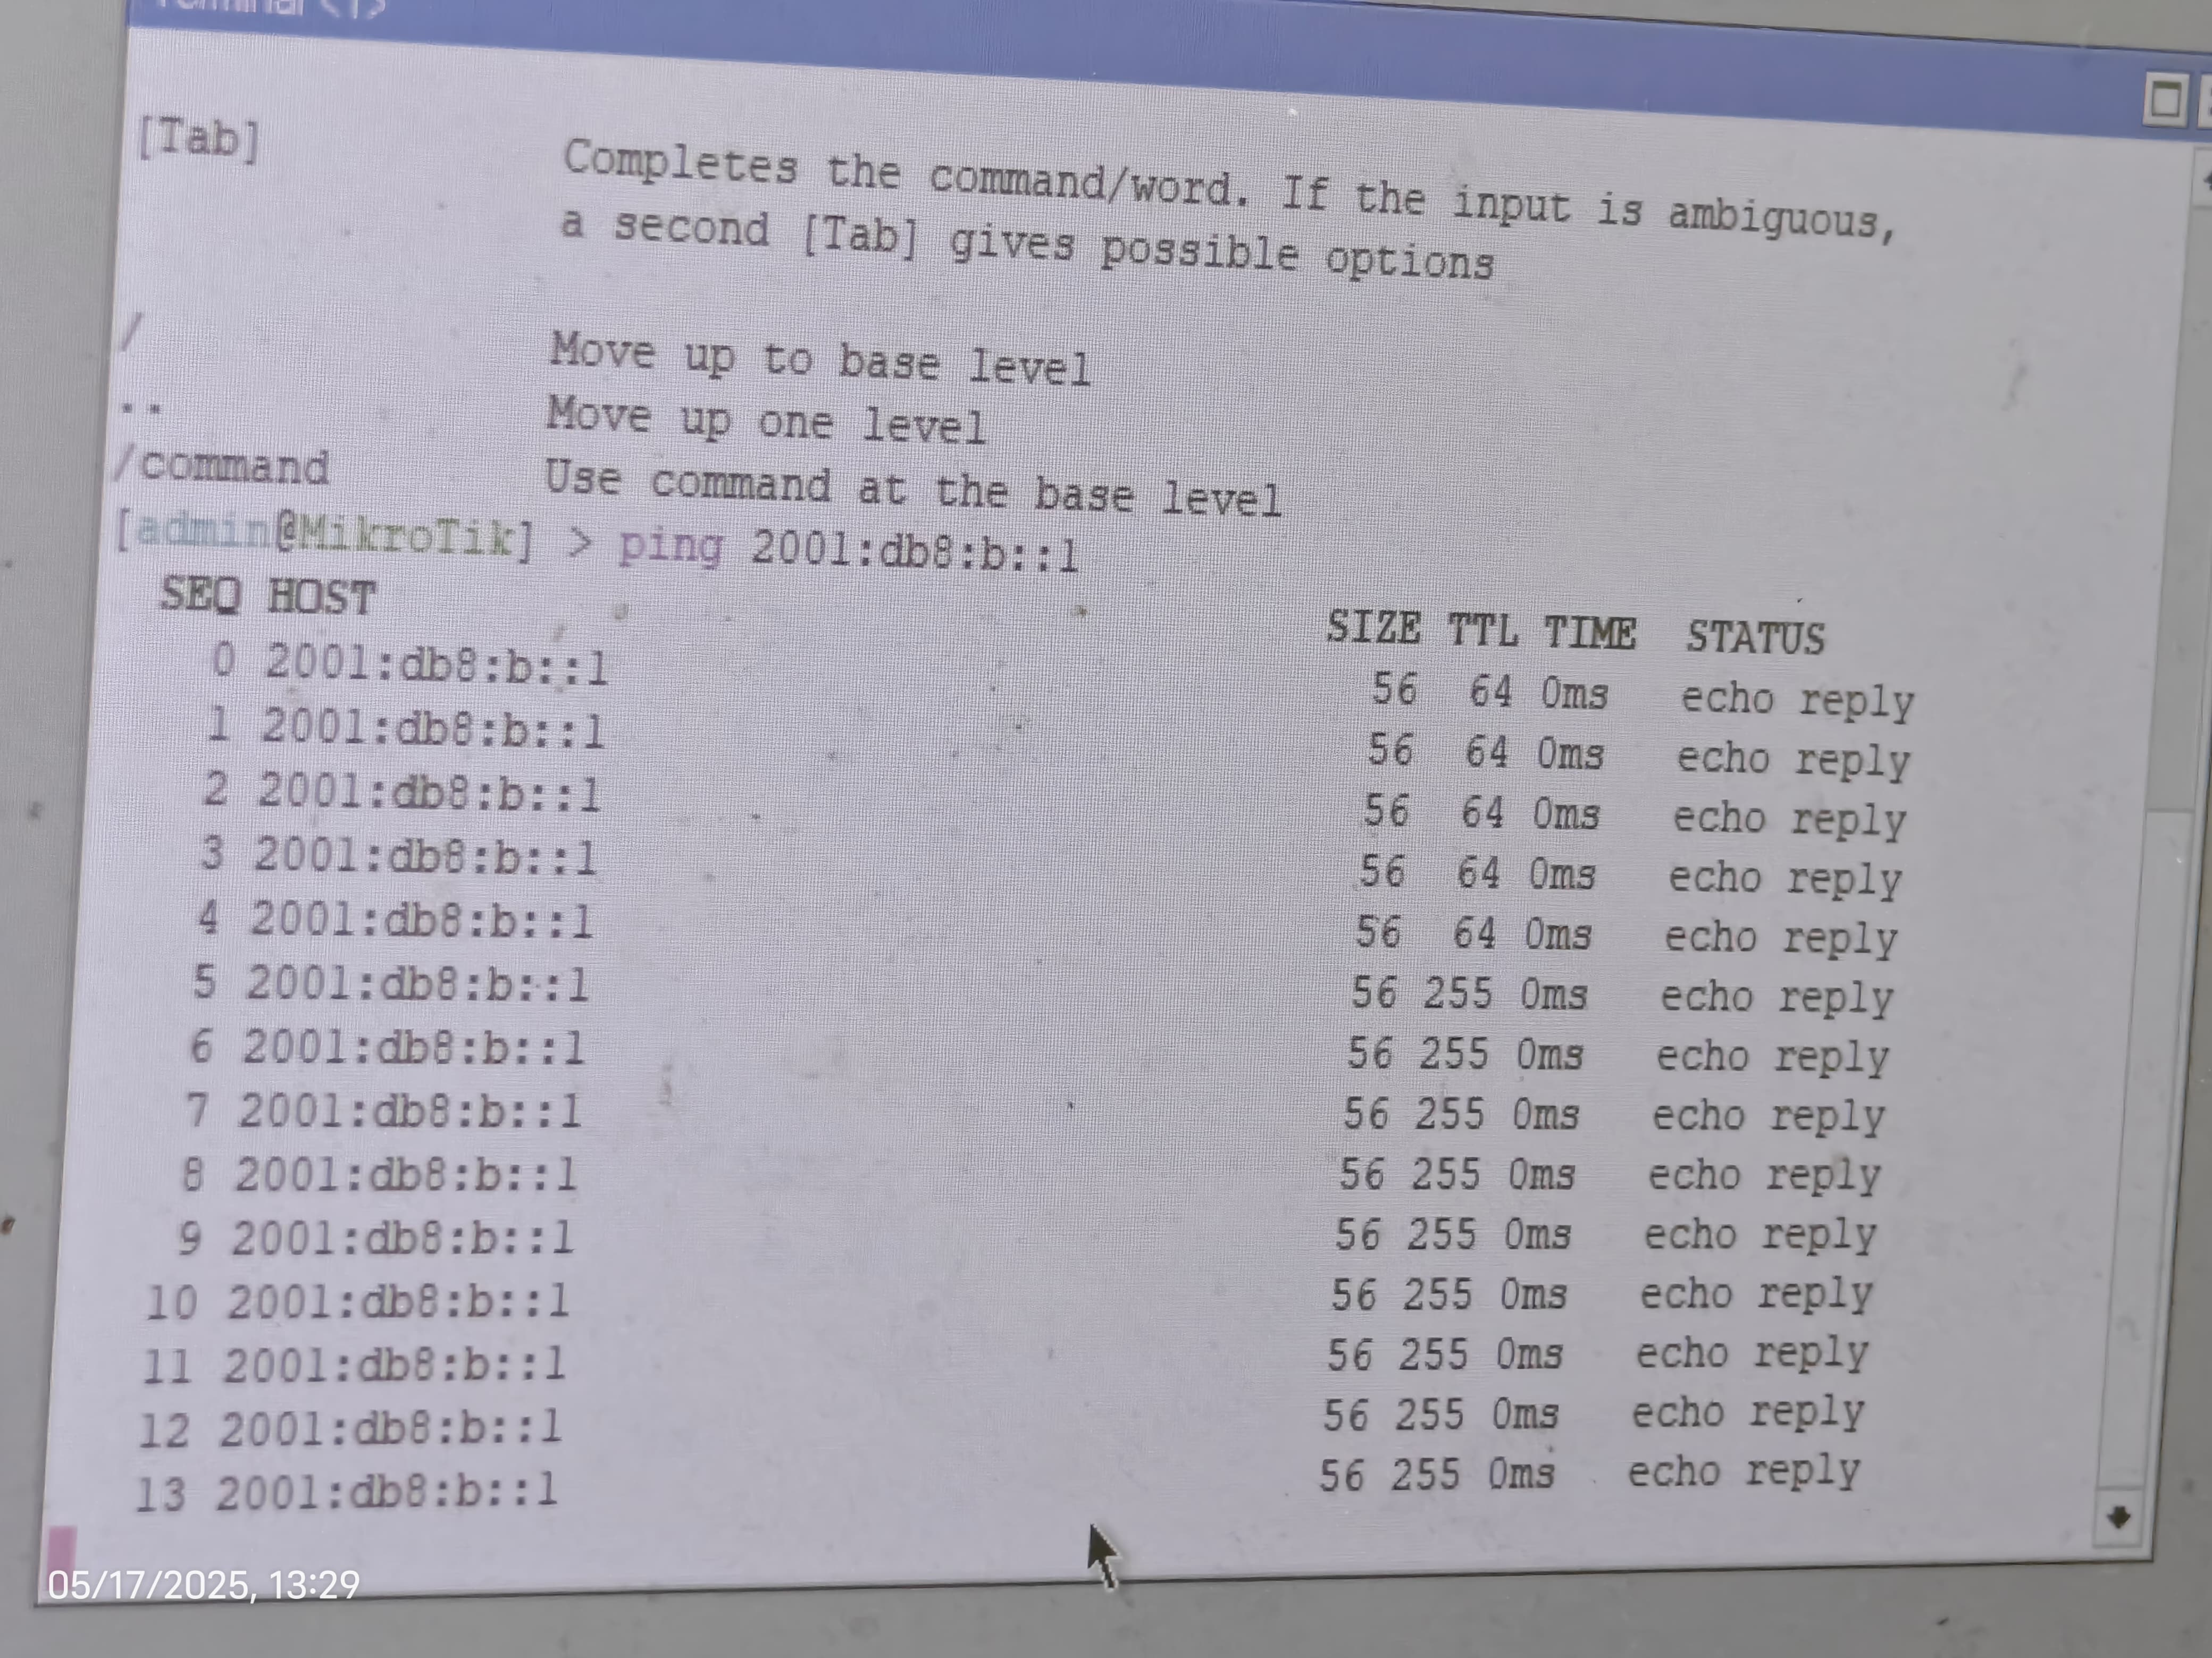
\includegraphics[width=0.48\textwidth]{img/A5.jpeg}
    \caption{Uji \textit{ping} pada PC2}
    \label{fig:a5}
\end{figure}

\begin{figure}[H]
    \centering
    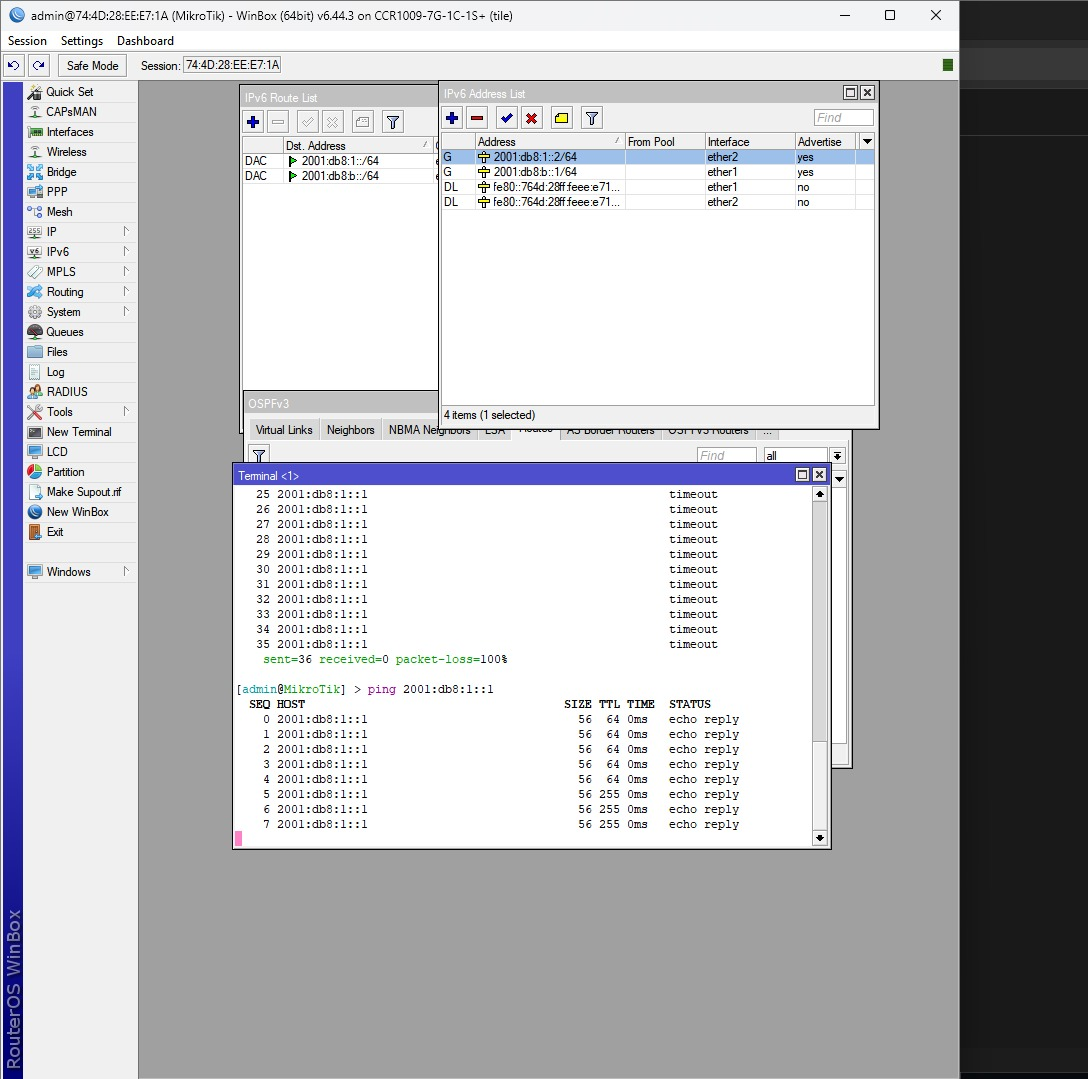
\includegraphics[width=0.48\textwidth]{img/A3.jpeg}
    \caption{Konfigurasi dan uji \textit{ping} pada PC1}
    \label{fig:a3}
\end{figure}
\end{enumerate}
\newpage
\section{Analisis Hasil Percobaan}

\subsection{Routing Statis IPv6}
 Sebelum melakukan praktikum, router direset konfigurasinya. kemudian dilakukan konfigurasi ulang dengan konfigurasi sebagai berikut.
	\textbf{Antarmuka Ether1 (antar-router):}\\
		$\bullet$ Router 1: \texttt{2001:db8:1::1/64}\\
		$\bullet$ Router 2: \texttt{2001:db8:1::2/64}\\
	\textbf{Antarmuka Ether2 (jaringan LAN):}\\
		$\bullet$ Router 1: \texttt{2001:db8:a::1/64}\\
		$\bullet$ Router 2: \texttt{2001:db8:b::1/64}\\
Serta IPv6 dari PC1 dan PC2 diatur sebagai berikut\\
\textbf{Konfigurasi IPv6 PC}\\
$\bullet$ PC1: \texttt{2001:db8:a::100/64}\\
Gateway: 2001:db8:a::1\\
DNS; 2001:4860:4860::8888\\ 
$\bullet$ PC2:\texttt{2001:db8:b::100/64}\\
Gateway: 2001:db8:b::1\\
DNS: 2001:4860:4860::8888

Selanjutnya, rute statis ditambahkan untuk memungkinkan komunikasi antar jaringan LAN yang terhubung ke masing-masing router:
\begin{itemize}
	\item Pada Router\,1, ditambahkan rute ke jaringan \texttt{2001:db8:b::/64} melalui \textit{gateway} \texttt{2001:db8:1::2}.
	\item Pada Router\,2, ditambahkan rute ke jaringan \texttt{2001:db8:a::/64} melalui \textit{gateway} \texttt{2001:db8:1::1}.
\end{itemize}

Setelah konfigurasi selesai, dilakukan pengujian konektivitas menggunakan perintah \textit{ping} antar-router dan antar perangkat di jaringan LAN. Ketika dilakukan ping dari PC1 ke Router 2 dan dari PC2 ke Router 1, dan telah berhasil, kemudian dilakukan tes ping antar PC, Pada PC1 \textit{ping} antar PC telah berhasil,namun pada awalnya pada PC2 setelah berhasil melakukan \textit{ping} ke router 1, dicoba ping PC1 namun gagal. Kemudian dicoba untuk melakukan \textit{ping} pada command prompt dan berhasil dan ketika dicoba lagi di terminal winbox tetap gagal. Karena di command prompt dicoba berulang-ulang dan dapat menghasilkan hasil yang baik, maka dianggap berhasil. Artinya routing statis IPv6 telah berhasil dilakukan.


\subsection{Routing Dinamis IPv6}

Untuk routing dinamis perlu dibuat protokol routing dinamis. Digunakanlah protokol OSPFv3 yang dikonfigurasi sebagai berikut \textit{Router ID} ditetapkan menjadi \texttt{1.1.1.1} (Router\,1) dan \texttt{2.2.2.2} (Router\,2) dengan \texttt{Area ID 0.0.0.0}. Setelah status \textit{Neighbor} OSPF terpantau aktif, dilakukan tes \textit{ping} antara PC1 ke Router 2, dari PC2 ke router 1 dan antaar PC. Sama seperti pada Routing statis, Awalnya pada PC2 setelah berhasil melakukan \textit{ping} ke router 1, dicoba ping PC1 namun gagal. Kemudian dicoba untuk melakukan \textit{ping} pada command prompt dan berhasil dan ketika dicoba lagi di terminal winbox tetap gagal. Karena di command prompt dicoba berulang-ulang dan dapat menghasilkan hasil yang baik, maka dianggap berhasil. Artinya routing dinamis IPv6 telah berhasil dilakukan.

\newpage
\section{Hasil Tugas Modul}

Tugas modul mensyaratkan demonstrasi \textit{routing statis} dan \textit{routing dinamis} IPv6 menggunakan Cisco Packet Tracer.

\subsection{Routing Statis}
\begin{figure}[H]
	\centering
	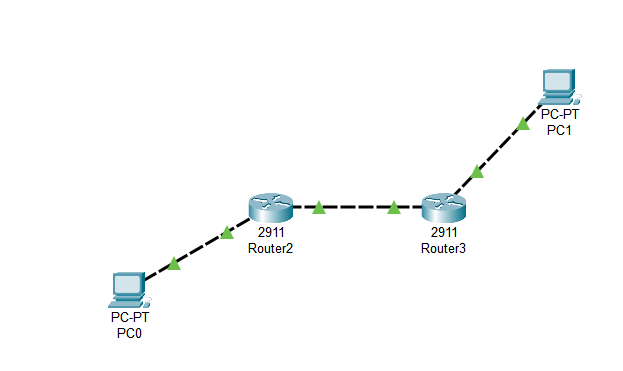
\includegraphics[width=0.48\textwidth]{img/Topologistatis.png}
	\caption{Simulasi routing statis}
	\label{fig:tumod1}
\end{figure}

setelah dibuat topologinya, kemudian diatur IP pada PC.\\
$\bullet$ IPv6 PC 0 = 2001:1::10/64\\
Default Gateway = 2001:1::1\\
$\bullet$ IPv6 PC 1 = 2001:3::10/64\\
Default Gateway: 2001:3::1\\

Kemudian diatur IPv6 pada router, karena pada cisco packet tracer tidak bisa mengatur IPv6 secara langsung maka harus digunakan CLI, seperti berikut

\textbf{Router2}\\
\begin{verbatim}
	Router> enable
	Router# configure terminal
	Router(config)# ipv6 unicast-routing
	Router(config)# interface gigabitEthernet0/0
	Router(config-if)# ipv6 address 2001:1::1/64
	Router(config-if)# no shutdown
	Router(config-if)# exit
	Router(config)# interface gigabitEthernet0/1
	Router(config-if)# ipv6 address 2001:2::1/64
	Router(config-if)# no shutdown
	Router(config-if)# exit
\end{verbatim}
\textbf{Router3}
\begin{verbatim}
	Router> enable
	Router# configure terminal
	Router(config)# ipv6 unicast-routing
	Router(config)# interface gigabitEthernet0/0
	Router(config-if)# ipv6 address 2001:2::2/64
	Router(config-if)# no shutdown
	Router(config-if)# exit
	Router(config)# interface gigabitEthernet0/1
	Router(config-if)# ipv6 address 2001:3::1/64
	Router(config-if)# no shutdown
	Router(config-if)# exit
\end{verbatim}

Kemudian dilakukan Routingnya pada PC0:
\begin{verbatim}
	Router(config)# ipv6 route 2001:3::/64 2001:2::2
\end{verbatim}
dan pada PC1:
\begin{verbatim}
	Router(config)# ipv6 route 2001:1::/64 2001:2::1
\end{verbatim}
ketika dicoba dilakukan ping, didapatkan berhasil. Artinya routing statis telaj berhasil dilakukan

\subsection{Routing dinamis}
\begin{figure}[H]
	\centering
	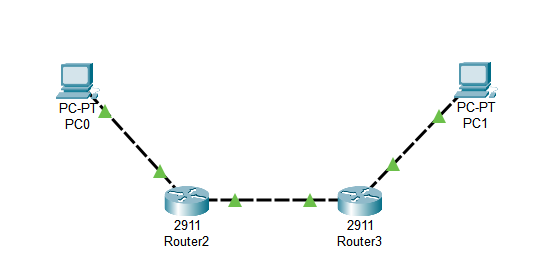
\includegraphics[width=0.48\textwidth]{img/Topologidinamis.png}
	\caption{Simulasi routing statis}
	\label{fig:tumod2}
\end{figure}

setelah dibuat topologinya, kemudian diatur IP pada PC.\\
$\bullet$ IPv6 PC 0 = 2001:1::10/64\\
Default Gateway = 2001:1::1\\
$\bullet$ IPv6 PC 1 = 2001:3::10/64\\
Default Gateway: 2001:3::1\\

Kemudian diatur IPv6 pada router, karena pada cisco packet tracer tidak bisa mengatur IPv6 secara langsung maka harus digunakan CLI, seperti berikut

\textbf{Router2}\\
\begin{verbatim}
	Router> enable
	Router# configure terminal
	Router(config)# ipv6 unicast-routing
	Router(config)# interface gigabitEthernet0/0
	Router(config-if)# ipv6 address 2001:1::1/64
	Router(config-if)# ipv6 ospf 1 area 0
	Router(config-if)# no shutdown
	Router(config-if)# exit
	Router(config)# interface gigabitEthernet0/1
	Router(config-if)# ipv6 address 2001:2::1/64
	Router(config-if)# ipv6  ipv6 ospf 1 area 0
	Router(config-if)# no shutdown
	Router(config-if)# exit
	Router(config)# ipv6  ipv6 ospf 1
	Router(config-rtr)# router-id 1.1.1.1
	exit
\end{verbatim}
\textbf{Router3}
\begin{verbatim}
	Router> enable
	Router# configure terminal
	Router(config)# ipv6 unicast-routing
	Router(config)# interface gigabitEthernet0/0
	Router(config-if)# ipv6 address 2001:2::2/64
	Router(config-if)# ipv6 ospf 1 area 0
	Router(config-if)# no shutdown
	Router(config-if)# exit
	Router(config)# interface gigabitEthernet0/1
	Router(config-if)# ipv6 address 2001:3::1/64
	Router(config-if)# ipv6 ospf 1 area 0
	Router(config-if)# no shutdown
	Router(config-if)# exit
	Router(config)# ipv6  ipv6 ospf 1
	Router(config-rtr)# router-id 2.2.2.2
	exit
\end{verbatim}
ketika dicoba dilakukan ping, didapatkan berhasil. Artinya routing dinamis telah berhasil dilakukan
\newpage
\section{Lampiran}

\subsection{Dokumentasi Saat Praktikum}

\begin{figure}[H]
    \centering
    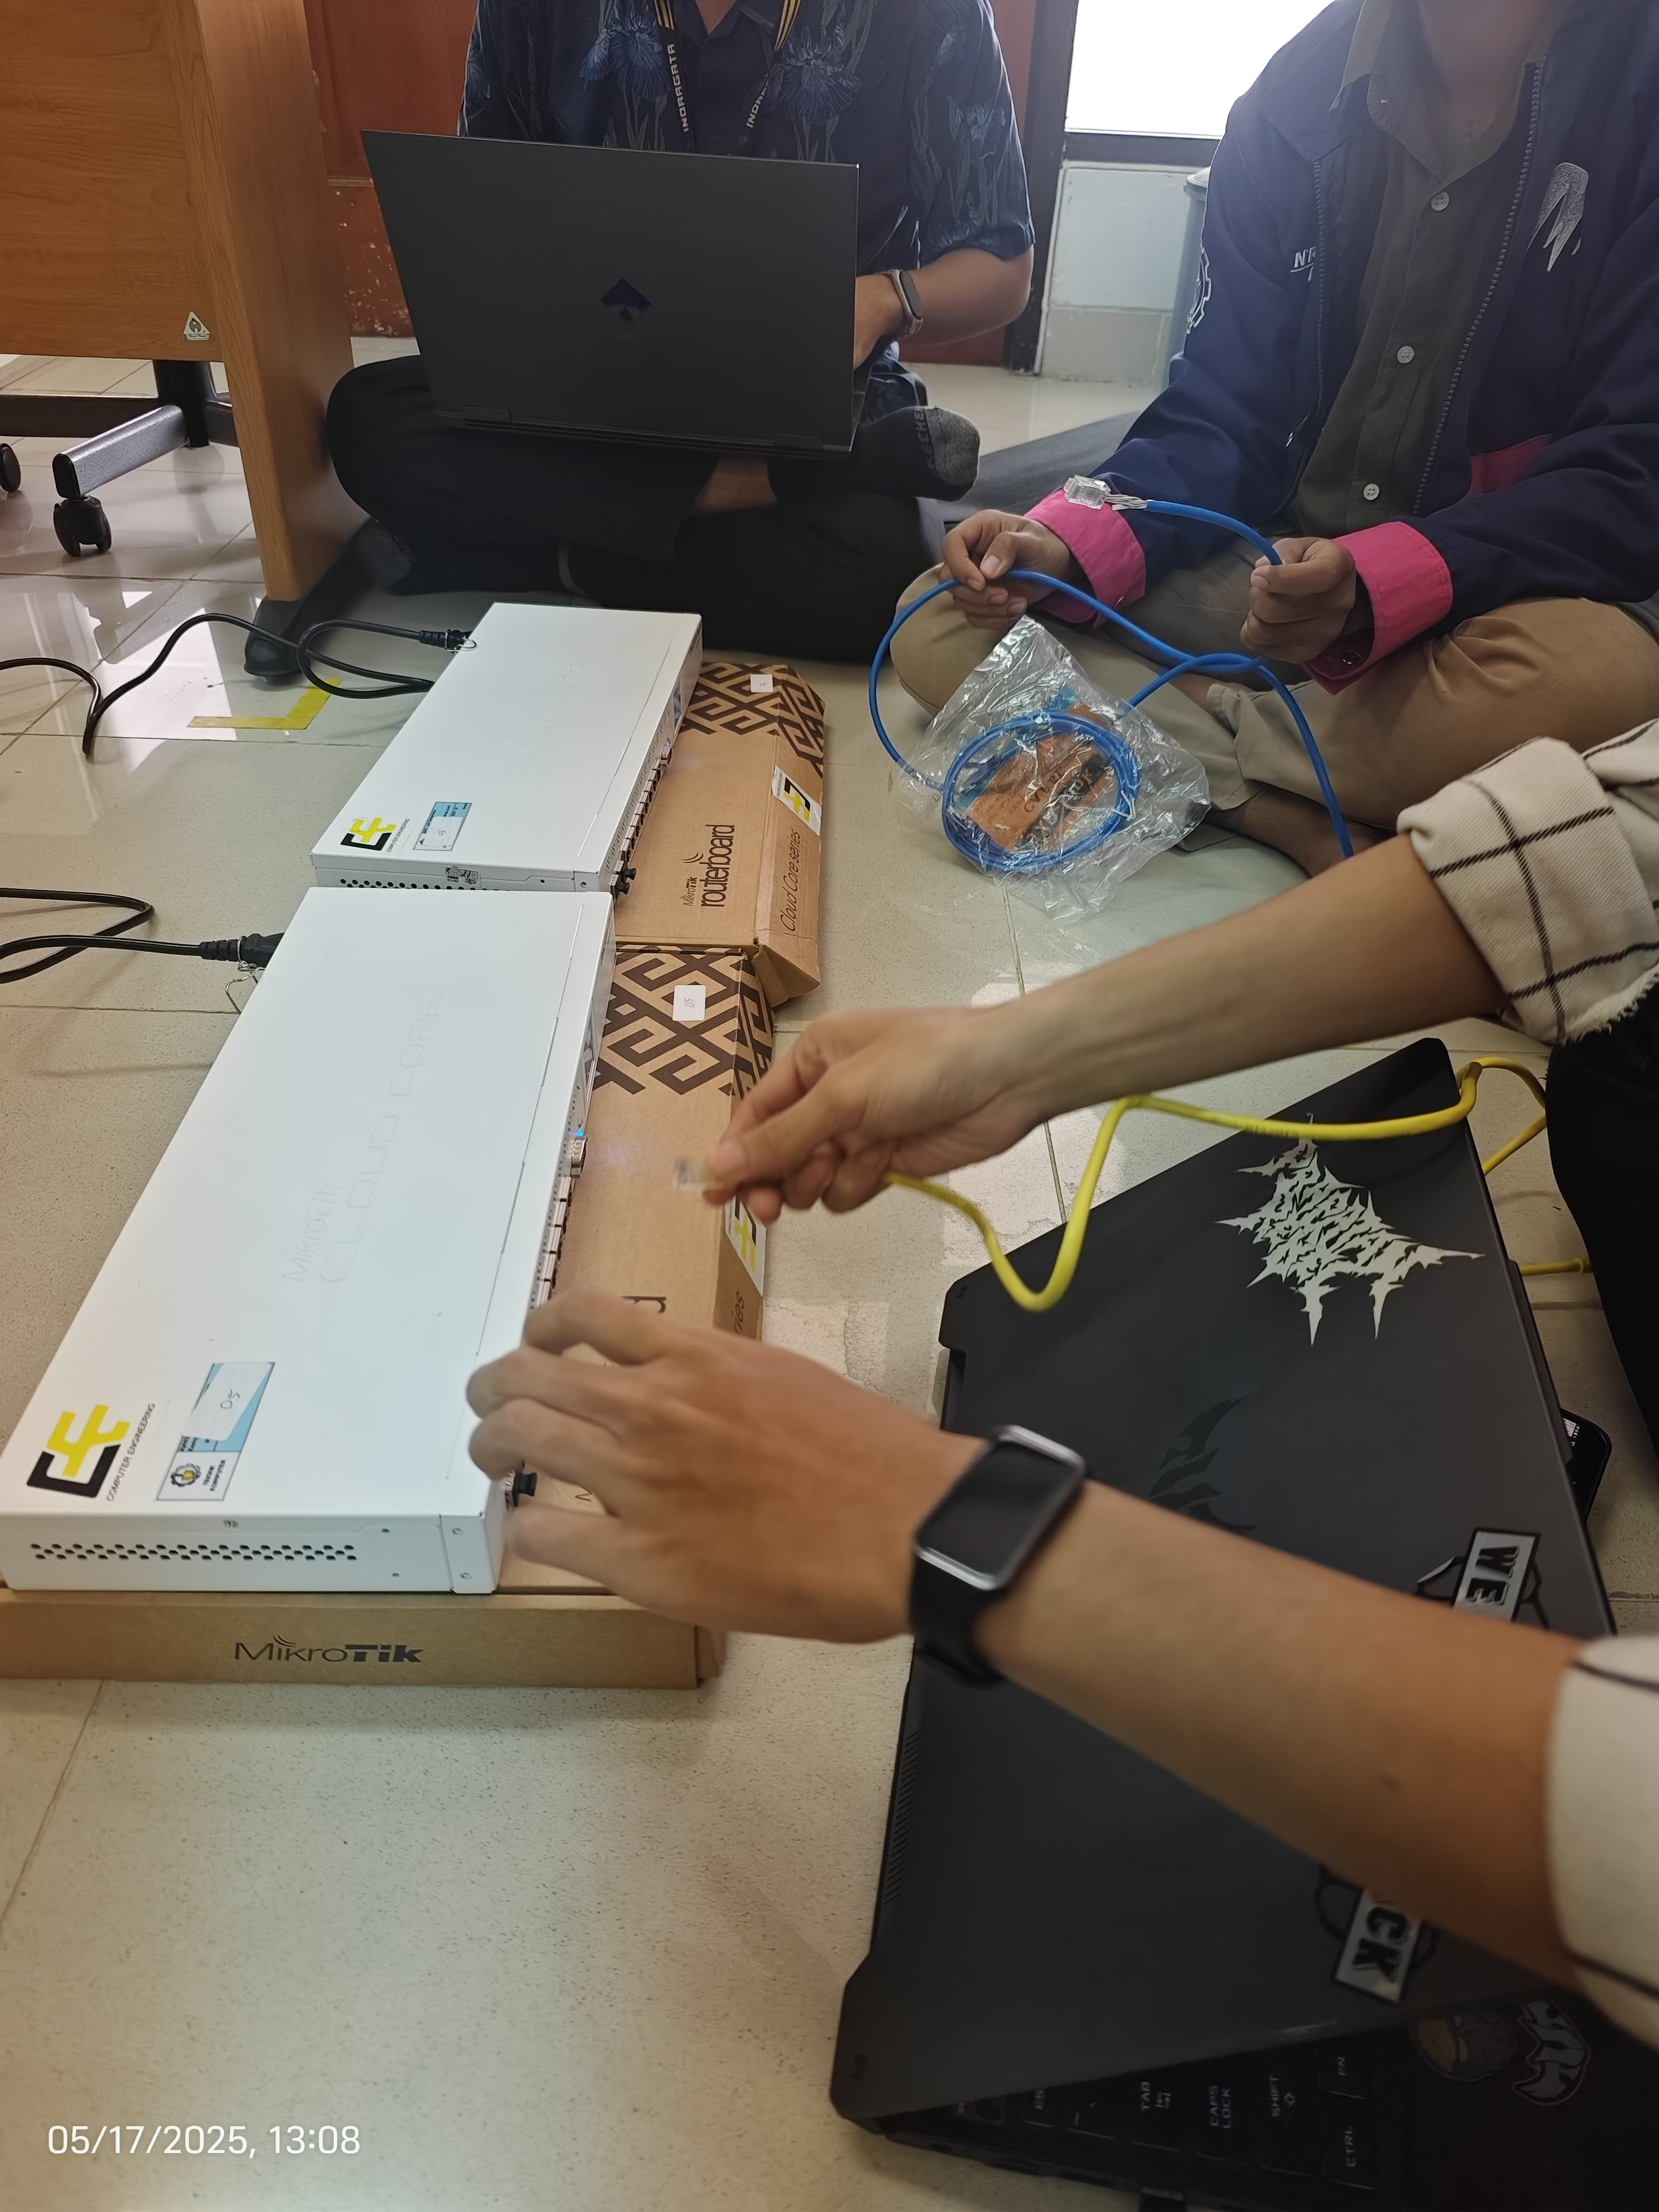
\includegraphics[width=0.48\textwidth]{img/Lampiran1.jpeg}
    \caption{Praktikan menyusun kabel}
    \label{fig:lmp1}
\end{figure}


